\documentclass{llncs}
\usepackage[noend]{algpseudocode}
\usepackage{subcaption}
\usepackage{subfig} 
\usepackage{usual}
\usepackage{graphicx}
\usepackage[rflt]{floatflt}
%\pagestyle{plain}
%
\begin{document}
\title{Plan Recovery in Reactive HTNs\\Using Symbolic Planning\vskip -10pt}

\author{Lydia Ould Ouali\inst{1}, Charles Rich\inst{2} \and
Nicolas Sabouret\inst{1} }

\institute{LIMSI-CNRS, UPR 3251, Orsay, France \\
Universit\'e Paris-Sud, Orsay, France \\
\email{\{ouldouali, nicolas.sabouret\}@limsi.fr}
\and
Worcester Polytechnic Institute\\ Worcester, Massachusetts, USA\\
\email{rich@wpi.edu}
}
\maketitle 
\begin{abstract}\vskip -20pt
  Building formal models of the world and using them to plan future
  action is a central problem in artificial intelligence.  In this
  work, we combine two well-known approaches to this problem, namely,
  reactive hierarchical task networks (HTNs) and symbolic linear
  planning.  The practical motivation for this hybrid approach was to
  recover from breakdowns in HTN execution by dynamically invoking
  symbolic planning.  This work also reflects, however, on the deeper
  issue of tradeoffs between procedural and symbolic modeling.  We
  have implemented our approach in a system that combines a reactive
  HTN engine, called Disco, with a STRIPS planner implemented in
  Prolog, and conducted a preliminary evaluation.
\end{abstract}

\section{Introduction}

\noindent Hierarchical task networks (HTNs) are widely used for
controlling intelligent agents and robots in complex, dynamic
environments.  There are many different formalizations and graphical
notations in use for HTNs.  In this paper we use the simple tree
notation shown in \fig{wind}, which we will explain in detail in
\sect{HTN}.  HTNs are typically hand-authored and can be quite large,
with five or more levels of task hierarchy and dozens or even
hundreds of tasks at the leaves.

All HTNs share the basic structure of decomposing tasks into sequences
(or sometimes partially ordered sets) of subtasks, with alternative
decompositions (sometimes called recipes) for different situations.
In addition to the decomposition tree structure, most HTNs also have
conditions, such as preconditions and postconditions, associated with
nodes in the tree to control execution of the HTN.

HTNs were originally a hierarchical extension of classical linear
(e.g., STRIPS \cite{Strips}) plans, and as in classical plans, the
conditions associated with tasks were {\em symbolic}, i.e., they were
written in some kind of formal logic and logical inference was used to
reason about them.  Later, in response to the difficulties of symbolic
modeling (see \sect{modeling}) a variant, called {\em reactive} HTNs,
was developed in which the conditions are {\em procedural}, i.e., they
are written in a programming language and evaluated by the appropriate
programming language interpreter.  The idea of reactive HTNs has also
been used in game development, where they are called behavior
trees.\footnote{See
  \url{http://aigamedev.com/open/article/popular-behavior-tree-design}}

This work is focused on reactive HTNs, and specifically on recovering
from breakdowns in their execution.  The basic idea is to add a small
proportion of symbolic conditions to a reactive HTN in order to
support a linear planner performing local plan
recovery. \sect{motivating} below starts with a simple, motivating
example.

The problem of plan recovery has been studied in symbolic HTNs (see
\cite{AyanEtAl2007_HOTRiDE,BoellaDamiano2002,VanDerKrogtDeWeerdt2005,WarfieldEtAl2007}).
This work is inspirational, but not directly relevant, because these
plan repair techniques rely upon {\em all} of the conditions in the
HTN being symbolically expressed, which obviates the use of a reactive
HTN.

Others have proposed adding some kind of symbolic planning to reactive
HTNs.  For example, Firby \cite{Firby1987} proposed using a planner to
reorder tasks in the HTN execution or to help choose between
alternative decompositions. Brom \cite{Brom2005} proposed using
planning to help execute tasks with time constraints.  However, no one
has yet developed a complete hybrid procedural/symbolic algorithm (see
\sect{algorithm}) similar to ours.

Finally, this work is preliminary because, although we have
implemented and tested our algorithm on synthetically generated data
(see \sect{evaluation}), how well it will work in practice is still an
open question.

\begin{figure}[t]
\centerline{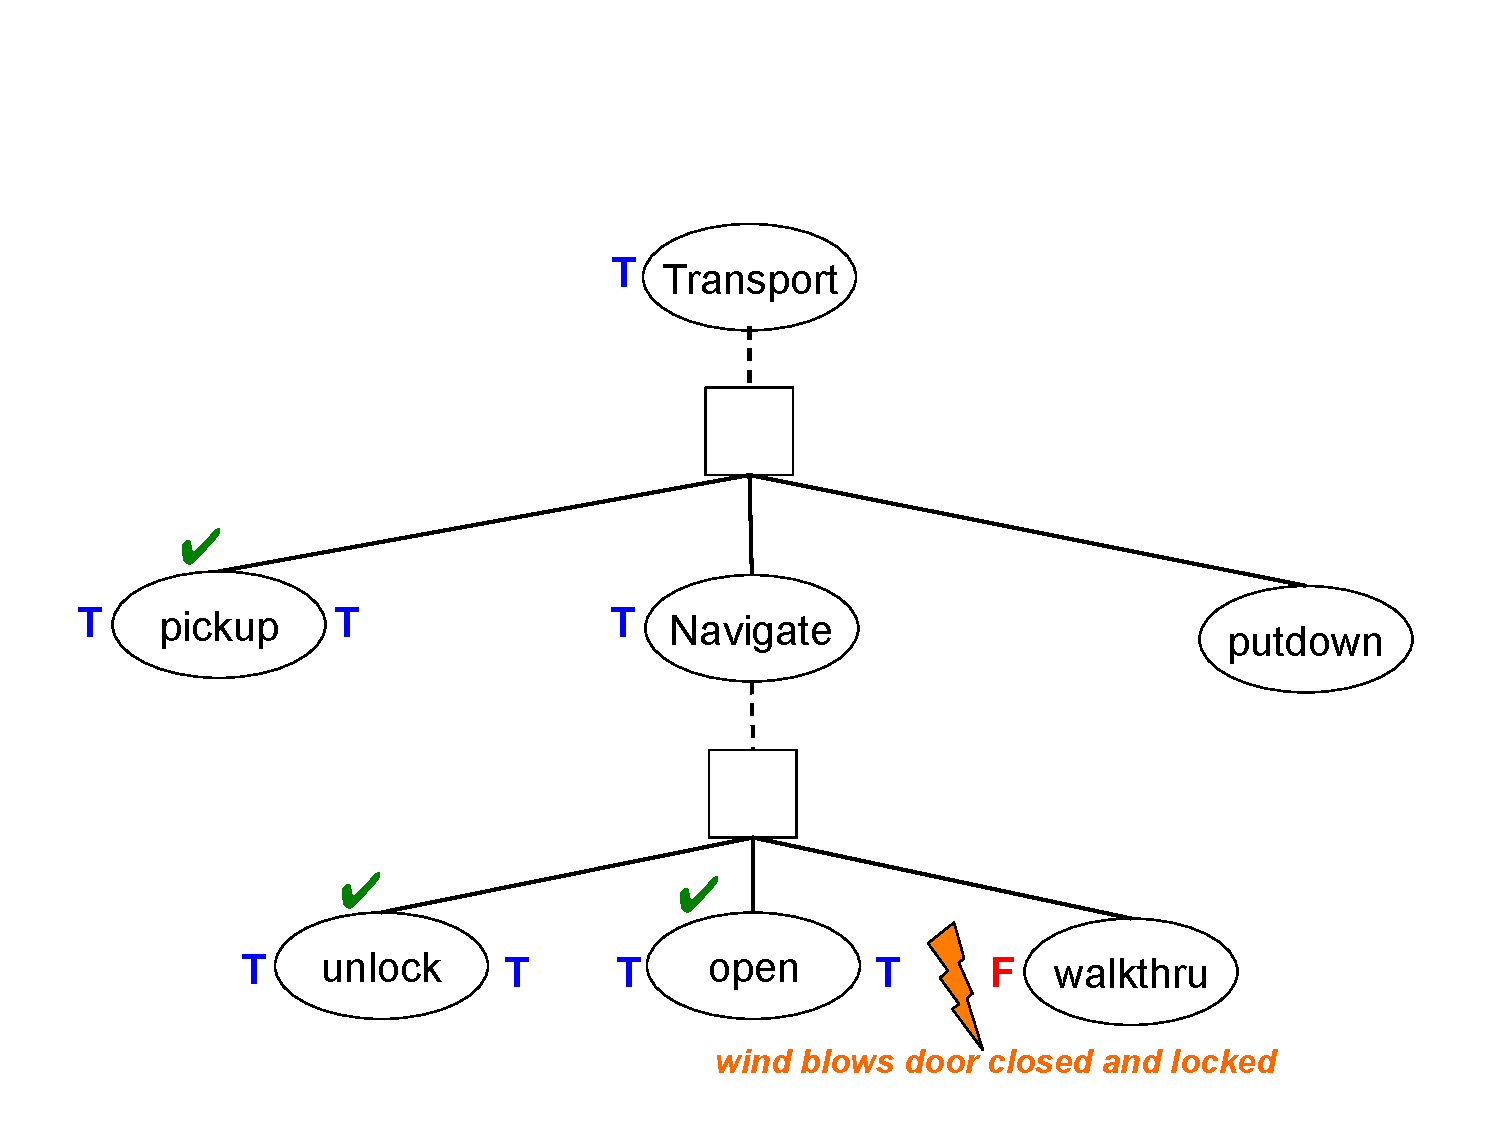
\includegraphics[width=3in]{figs/wind}}
\vskip 8pt
\defig{wind}{Breakdown in HTN execution after wind blows door closed and locked.  Check marks indicate successfully executed tasks;
``T'' indicates a condition that has been evaluated and returned true; ``F'' indicates a condition that has returned false.}
\end{figure}

\defsection{motivating}{A Motivating Example}

\noindent To further introduce and motivate our work, we first
consider a small, intuitive example of reactive HTN execution
breakdown and recovery.  The basic idea of this example, shown in
\fig{wind} is that a robot has been programmed using an HTN to
transport an object through a locked door.  In this HTN, the toplevel
task, Transport, is decomposed into three steps: pickup, Navigate and
putdown.  Navigate is further decomposed into three steps: unlock,
open and walkthrough.  Each of these tasks is represented by an oval in
\fig{wind}.  (The square boxes in the HTN are there to support
alternative decompositions, which can be ignored in this example.)

At the moment in time depicted in \fig{wind}, the robot has
successfully picked up the object, unlocked the door and opened it.
However, before the precondition of the walkthru step is evaluated,
the wind blows the door closed and the door locks.  The walkthru
precondition checks that the door is open and thus returns false.  At
this point, there are then no executable tasks in the HTN, which is
what we call a \emph{breakdown}.

Such breakdowns are not unusual in reactive HTNs, especially when they
are executing in complex, dynamic environments. In fact, something
similar to this actually happened recently to the winning robot in the
prestigious DARPA Robotics Challenge\footnote{\url{https://herox.com/news/148-the-darpa-robotics-challenge}} (emphasis added):
``However, team Schaft lost points when \emph{a gust of wind blew a
  door out of the robot's hand and the robot was unable to exit a
  vehicle} after navigated a driving course successfully.''  It can be
hard to anticipate all possible things that can go wrong; and trying to
incorporate all possible recovery plans into the HTN in advance can
lead to an explosion of programming effort.

\begin{figure}[t]
\centerline{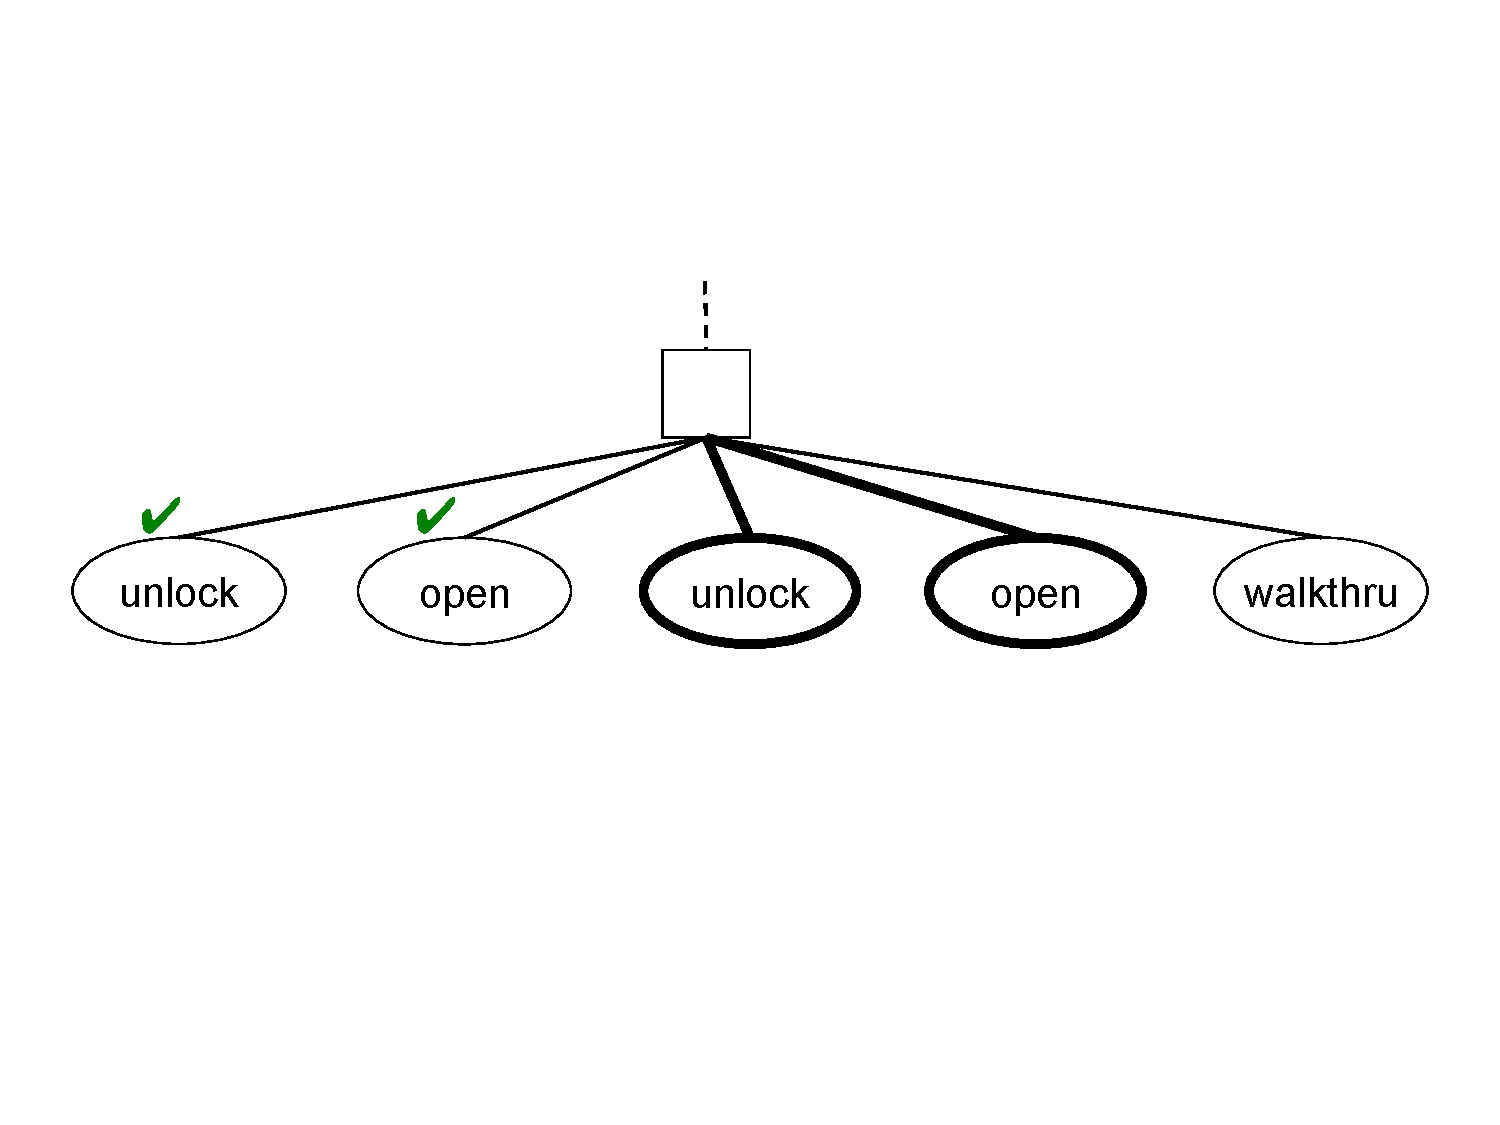
\includegraphics[width=3in]{figs/recover}}
\vskip 8pt
\defig{recover}{Sequence of two primitive tasks (in bold) added to plan for Navigate to recover from breakdown in \fig{wind}.}
\end{figure}

However, looking at this breakdown in particular, the recovery
solution, shown in \fig{recover}, is obvious, namely to unlock and
open the door.  Furthermore, this would be a trivial problem for a
symbolic linear (e.g., STRIPS) planner to solve if only the pre-
and postconditions of the relevant primitives were specified
symbolically.

In a reactive HTN, pre- and postconditions are written in a procedural
(programming) language and evaluated by the appropriate programming
language interpreter.  \fig{procedures} shows the relevant procedural
conditions in the Navigate plan as they might typically be written,
for example, in JavaScript.  For example, ``isOpen()'' would call code in
the robot's sensory system to check whether the door is currently
open.  In comparison, \fig{features} shows how the same primitive
tasks would typically be formalized for a STRIPS planner using
symbolic features.

Suppose that when the breakdown in \fig{wind} occurred, the HTN
execution engine somehow had available the symbolic modeling
knowledge shown in \fig{features}.  Recovering from the breakdown
could then be formulated as a STRIPS planning problem (see
\fig{planning}) in which the initial state is the \emph{current} world
state, i.e., the door is not open and is locked, and the final state is
the failed precondition of walkthru, i.e., the door is open.
Simple backward-chaining would then quickly find the solution sequence of
operators, namely unlock followed by open.  This recovery plan could
then be spliced into the HTN as shown in \fig{recover} and execution
could continue.

The goal of this paper is to generalize the solution to this example
problem into an application-independent plan recovery algorithm and
associated modeling methodology for reactive HTNs, as described in the
next two sections.

\begin{figure}[t]
\centering
\begin{subfigure}{2.3in}
\centerline{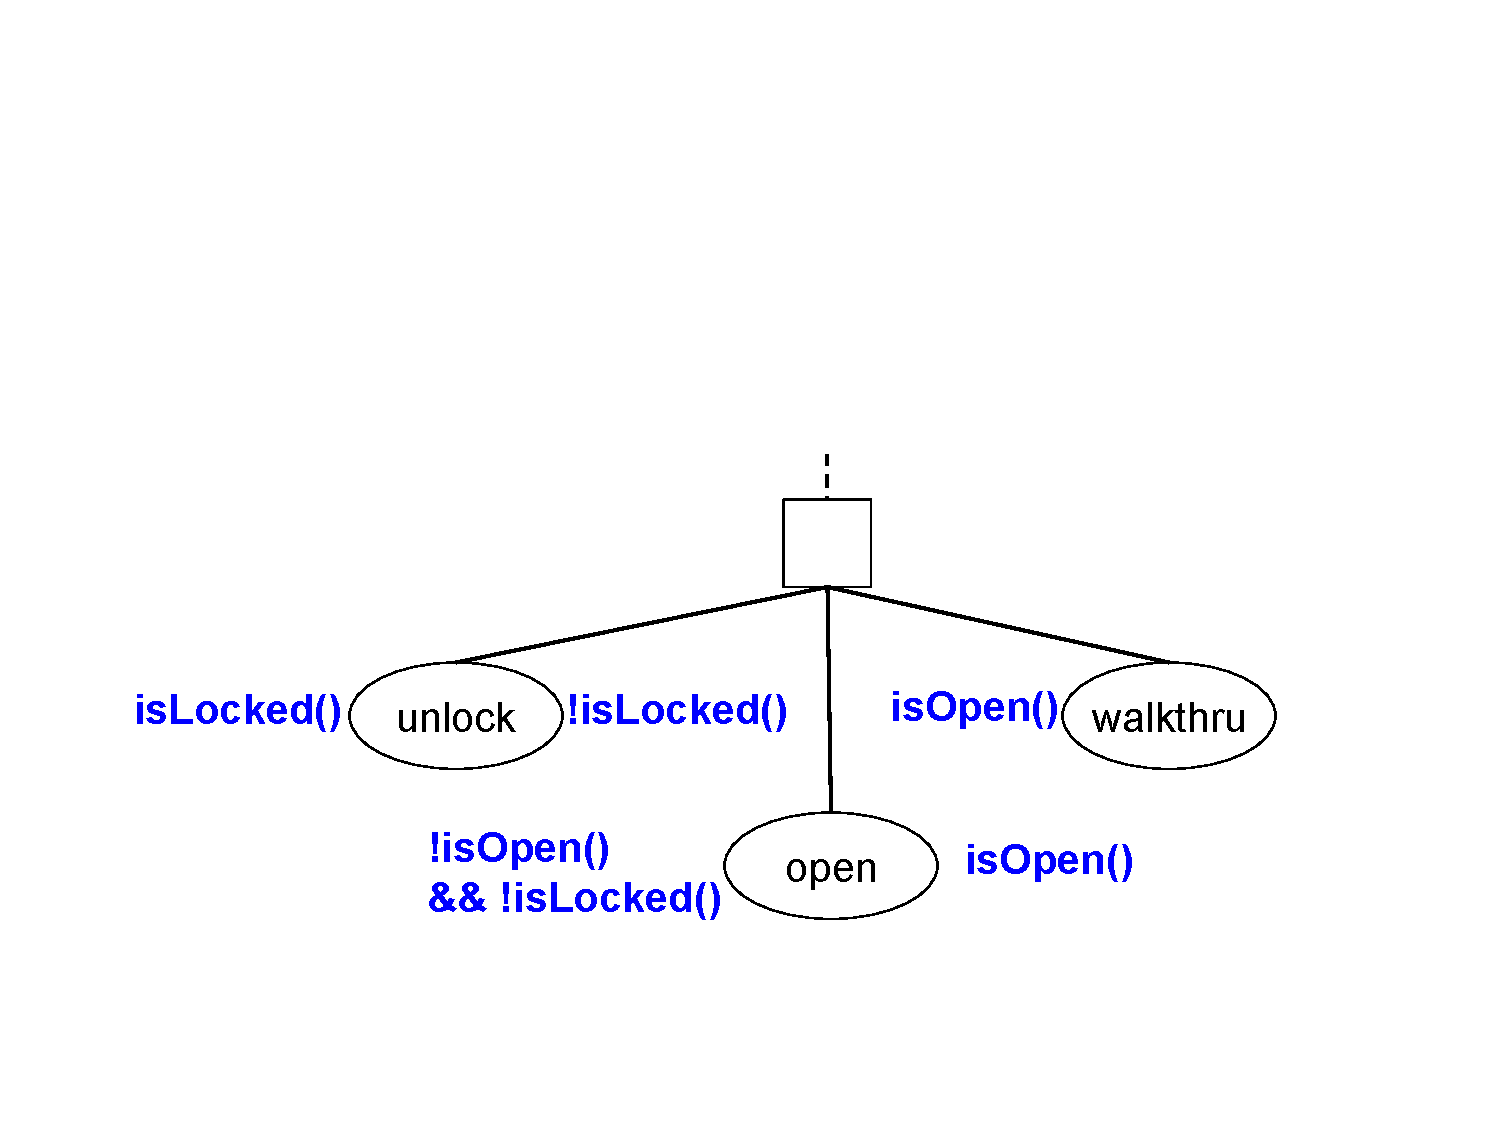
\includegraphics[width=2.4in]{figs/procedures}}
\vskip 8pt 
\defig{procedures}{Procedural conditions}
\end{subfigure}
\hfill
\begin{subfigure}{2.3in}
\centerline{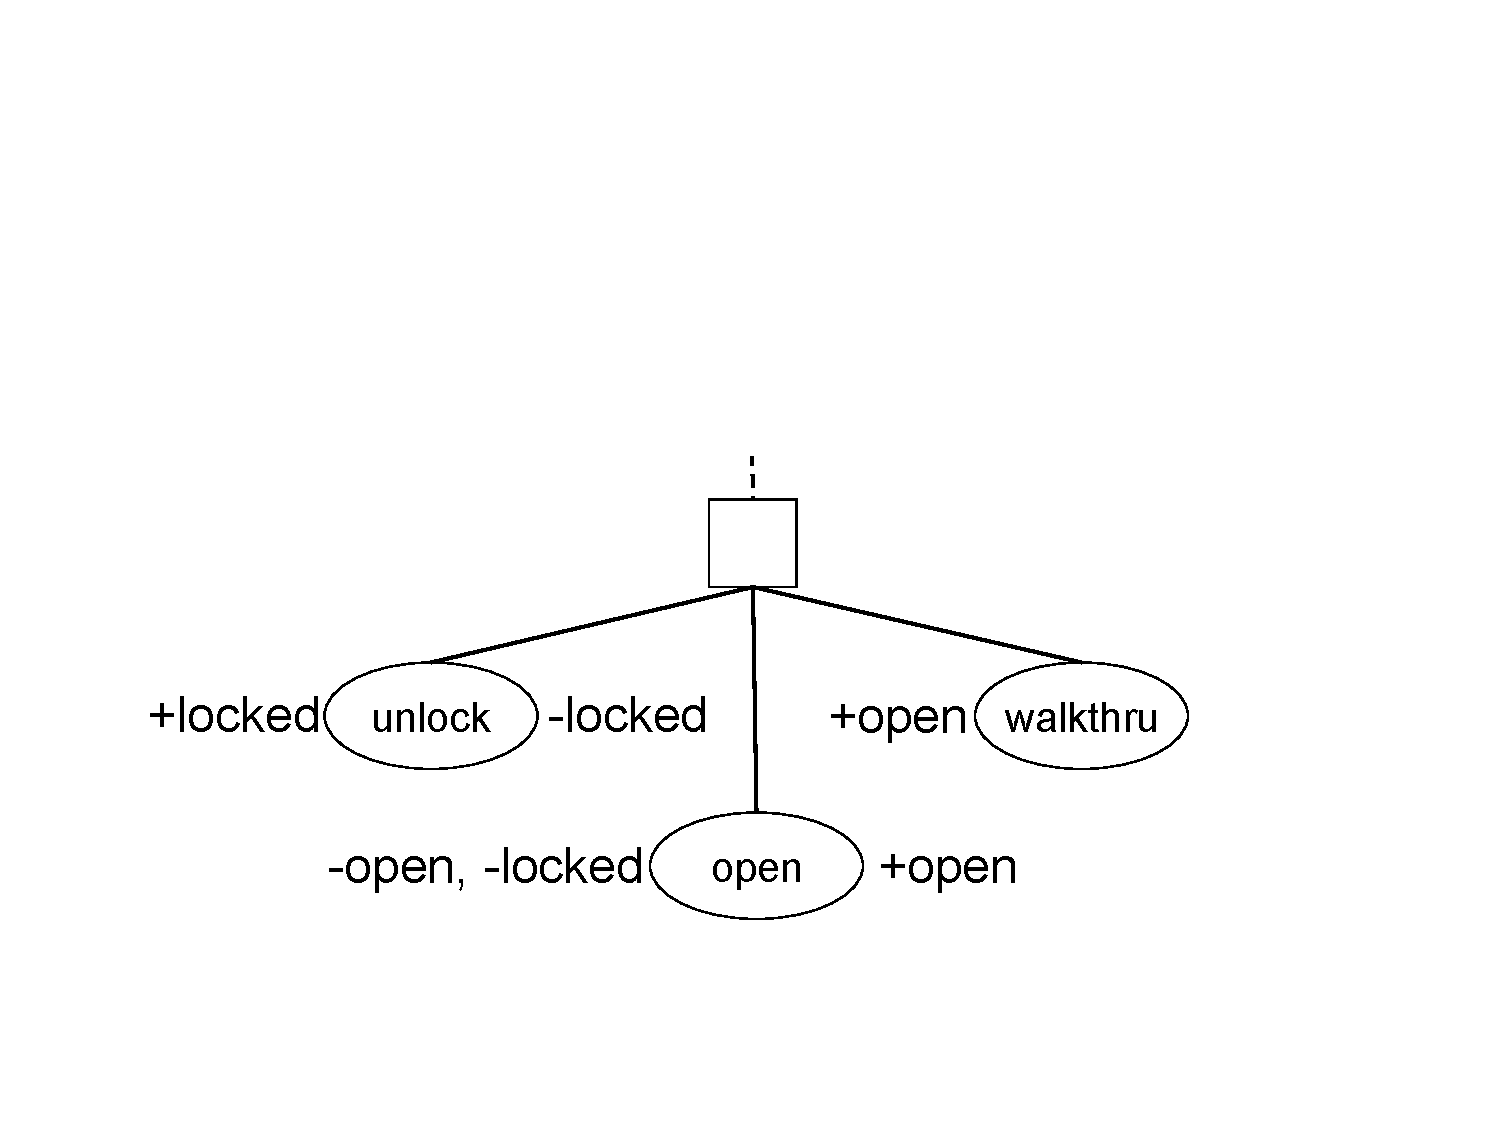
\includegraphics[width=2.4in]{figs/features}}
\vskip 8pt 
\defig{features}{Symbolic features for conditions}
\end{subfigure}
\vskip 8pt
\defig{comparison}{Procedural versus symbolic conditions for Navigate plan.}
\end{figure}
%
\begin{figure}[t]
\centerline{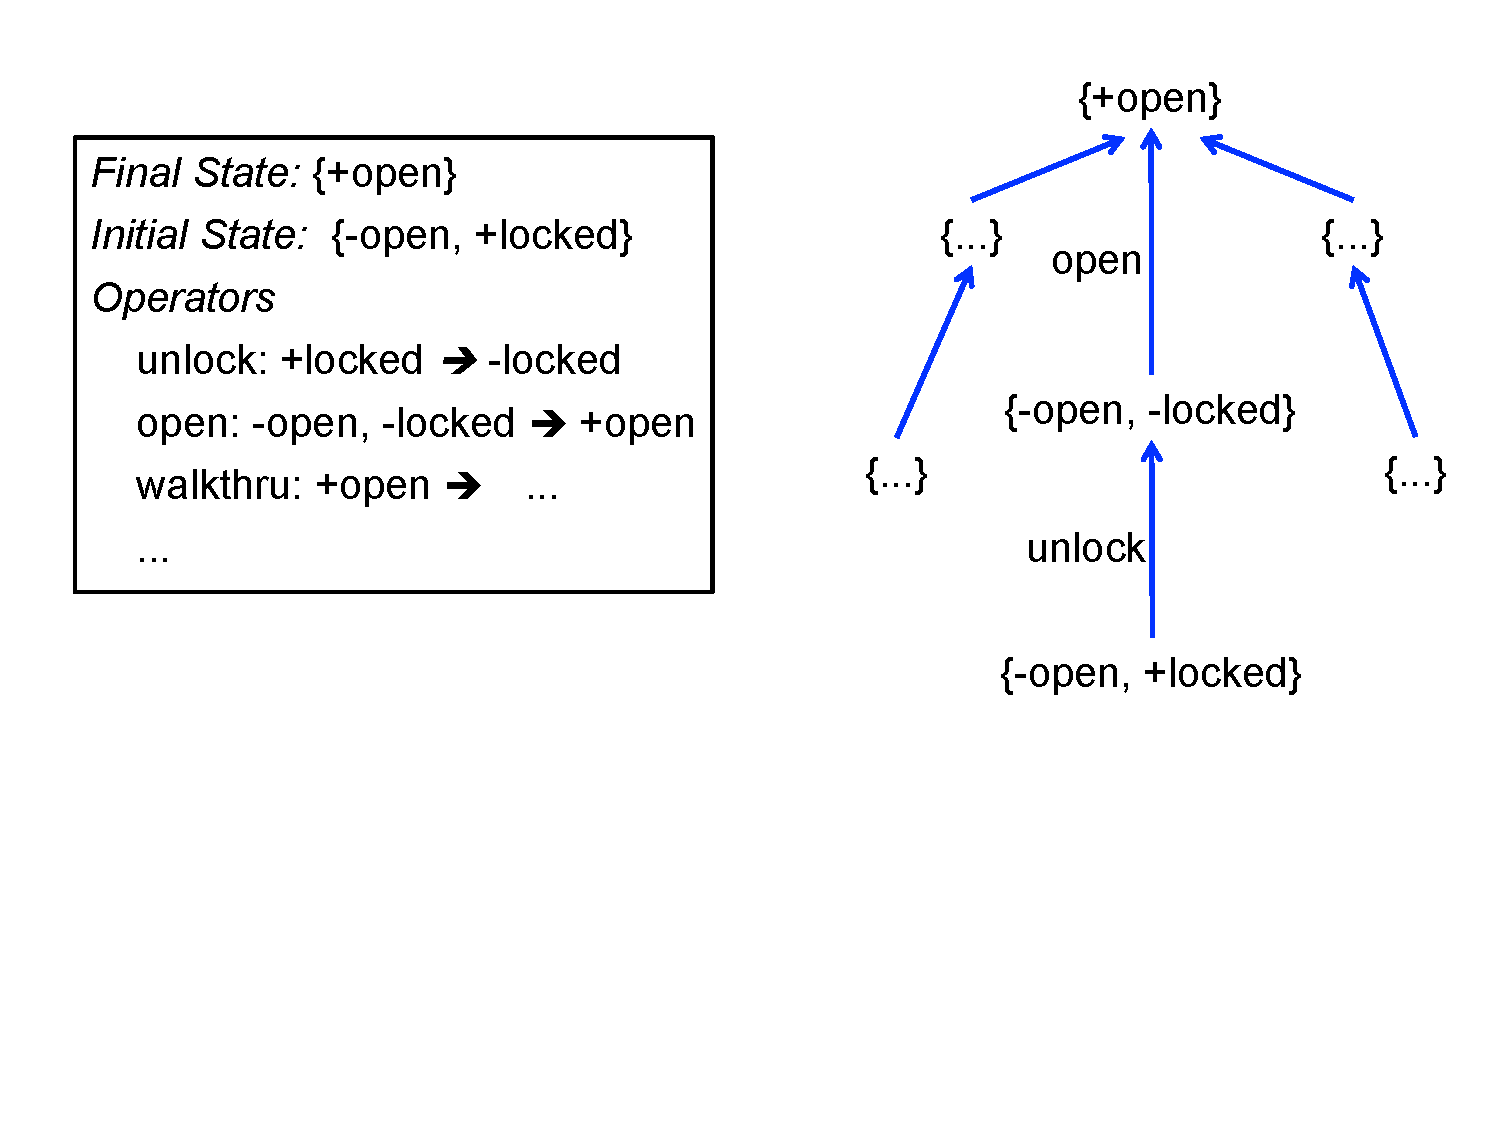
\includegraphics[width=3.7in]{figs/planning}}
\vskip 8pt
\defig{planning}{Recovery from breakdown in \fig{wind} as a STRIPS planning problem.}
\end{figure}

\defsection{modeling}{Procedural versus Symbolic Modeling}

\noindent A reasonable first question to ask after reading the
motivating example above is why not just use a symbolic planner
instead of an HTN to control the robot in the first place, and apply
well-known replanning approaches when a breakdown occurs?

Answering this question leads directly to the issue of modeling.
Symbolic planners, such as STRIPS, require \emph{complete and correct}
symbolic descriptions of all of the primitive tasks (operators) in the
problem domain.  Different planners use different symbolic formalisms
to represent this knowledge, such as the add/delete lists shown in
\fig{features}, PDDL \cite{PDDL}, and others.  However, what all
symbolic planners have in common is that if these symbolic
descriptions are incorrect or incomplete (relative to reality), then
the generated plans will fail---the poorer the correspondence to
reality, the less reliable the plans will be.

Unfortunately, artificial intelligence research has shown that
producing complete and correct symbolic descriptions of complex
real-world domains is extremely hard and, for practical purposes,
often impossible.  Certainly the textbook example in
\fig{planning} is easy to model symbolically, but no one participating
in the DARPA Robotics Challenge seriously considered symbolically
modeling the complete task domain.  

The difficulty of symbolic modeling is why reactive HTNs were
invented.  The knowledge in a reactive HTN is encoded in two places:
in the decomposition structure of the tree and in the code for the
procedural conditions (especially the applicability conditions for
decomposition choices, which will be explained in the next section).

So is it easier to model complex real-world domains using reactive
HTNs than symbolically?  As a practical matter, the answer appears to
be yes, since reactive HTNs are commonly used in such applications.
Our guess is that there are two main reasons for this.  First, it is
well known that hierarchy helps people organize their thinking to deal
with complexity.  Second, a procedural condition, such as a
precondition, is only applied to the \emph{current} world, whereas
symbolic descriptions are essentially axioms that must be true in all
possible worlds.

But of course, as we saw above, reactive HTNs can break down, which
leads us to the hybrid approach, described in the next section, in
which a reactive HTN is augmented with some symbolic conditions to aid
specifically with recovery.

\defsection{hybrid}{A Hybrid Approach}

\noindent In this section we generalize the motivating example in
\sect{motivating} in two ways by considering: (1) other types of
breakdowns and (2) a larger set of possible final states.  We will
first present a general plan recovery algorithm and then discuss the
modeling methodology that goes along with it.

\defsubsection{HTN}{Reactive HTNs}

\noindent For the purpose of this work, a reactive HTN, such as the
general example in \fig{precondition}, is formally a bipartite tree
with alternating levels of {\em task} nodes (shown as circles or
ovals) and {\em decomposition} (recipe) nodes (shown as squares), with
a task node at the root and task nodes at the leaves.  The tasks at
the leaves are called {\em primitive}; the other tasks are called {\em
  abstract}.

Associated with the nodes of the tree are three kinds of
boolean-valued procedures, each of what are evaluated in the current
world state.  Task nodes have an optional {\em precondition} and/or
{\em postcondition}.  Every decomposition node has an {\em
  applicability condition}.

Reactive HTNs are basically a kind of and/or tree, where the task
nodes are ``and'' and the decomposition nodes are ``or.''  Execution
is a depth-first, left-to-right traversal of the tree starting at the
root, with various conditions being evaluated along the way, as
described below.

If the current execution node is a task, then its precondition, if
any, is first evaluated.  If the precondition returns false, then
execution is halted (a breakdown); otherwise execution continues.  If
the task is primitive, then it is directly executed (typically
changing the world state); otherwise (i.e., for abstract tasks) the
applicability conditions of the children (decomposition) nodes are
evaluated in order until the first one that returns true---execution
continues with this decomposition node.  If all of the applicability
conditions of the children return false, then execution is halted (a
breakdown).

When execution of a task node is completed, its postcondition, if any,
is evaluated.  If the postcondition returns false, then execution is
halted (a breakdown); otherwise execution continues.

If the current execution node is a decomposition, then the children
(task) nodes are executed in order.

\begin{figure}[t]
\centering
\begin{subfigure}{2.1in}
\centerline{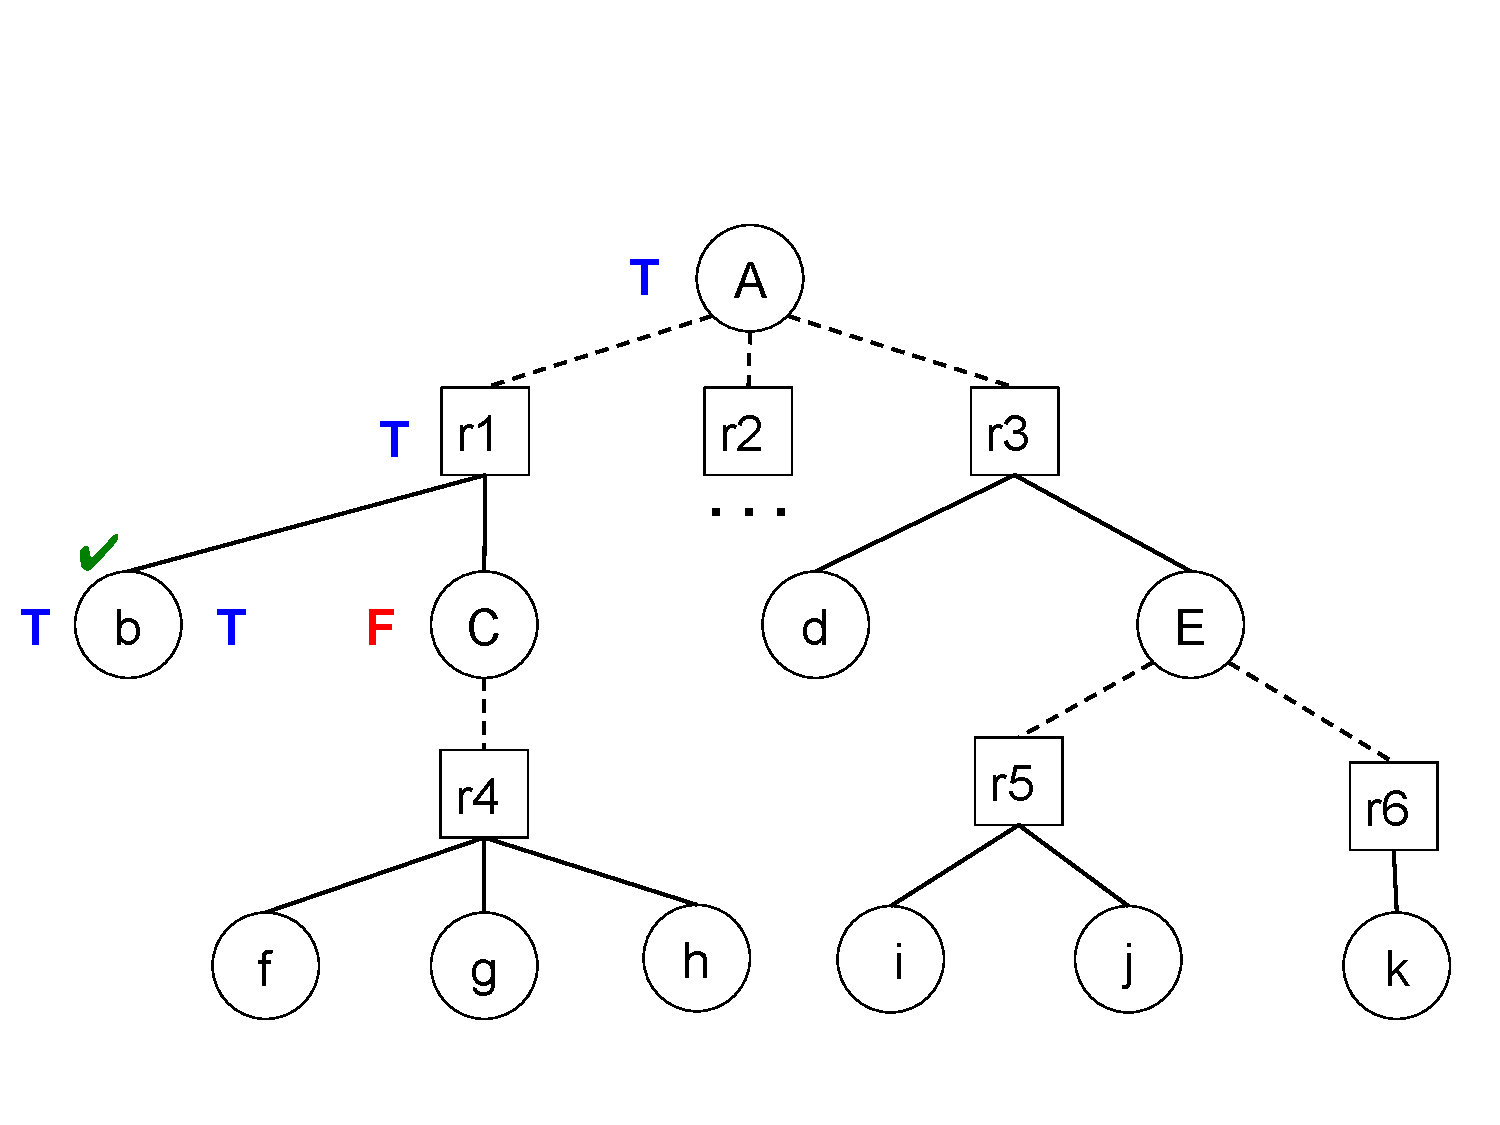
\includegraphics[height=1.3in]{figs/precondition}}
\vskip 8pt 
\defig{precondition}{Failed precondition}
\end{subfigure}
\hfill
\begin{subfigure}{1.4in}
\centerline{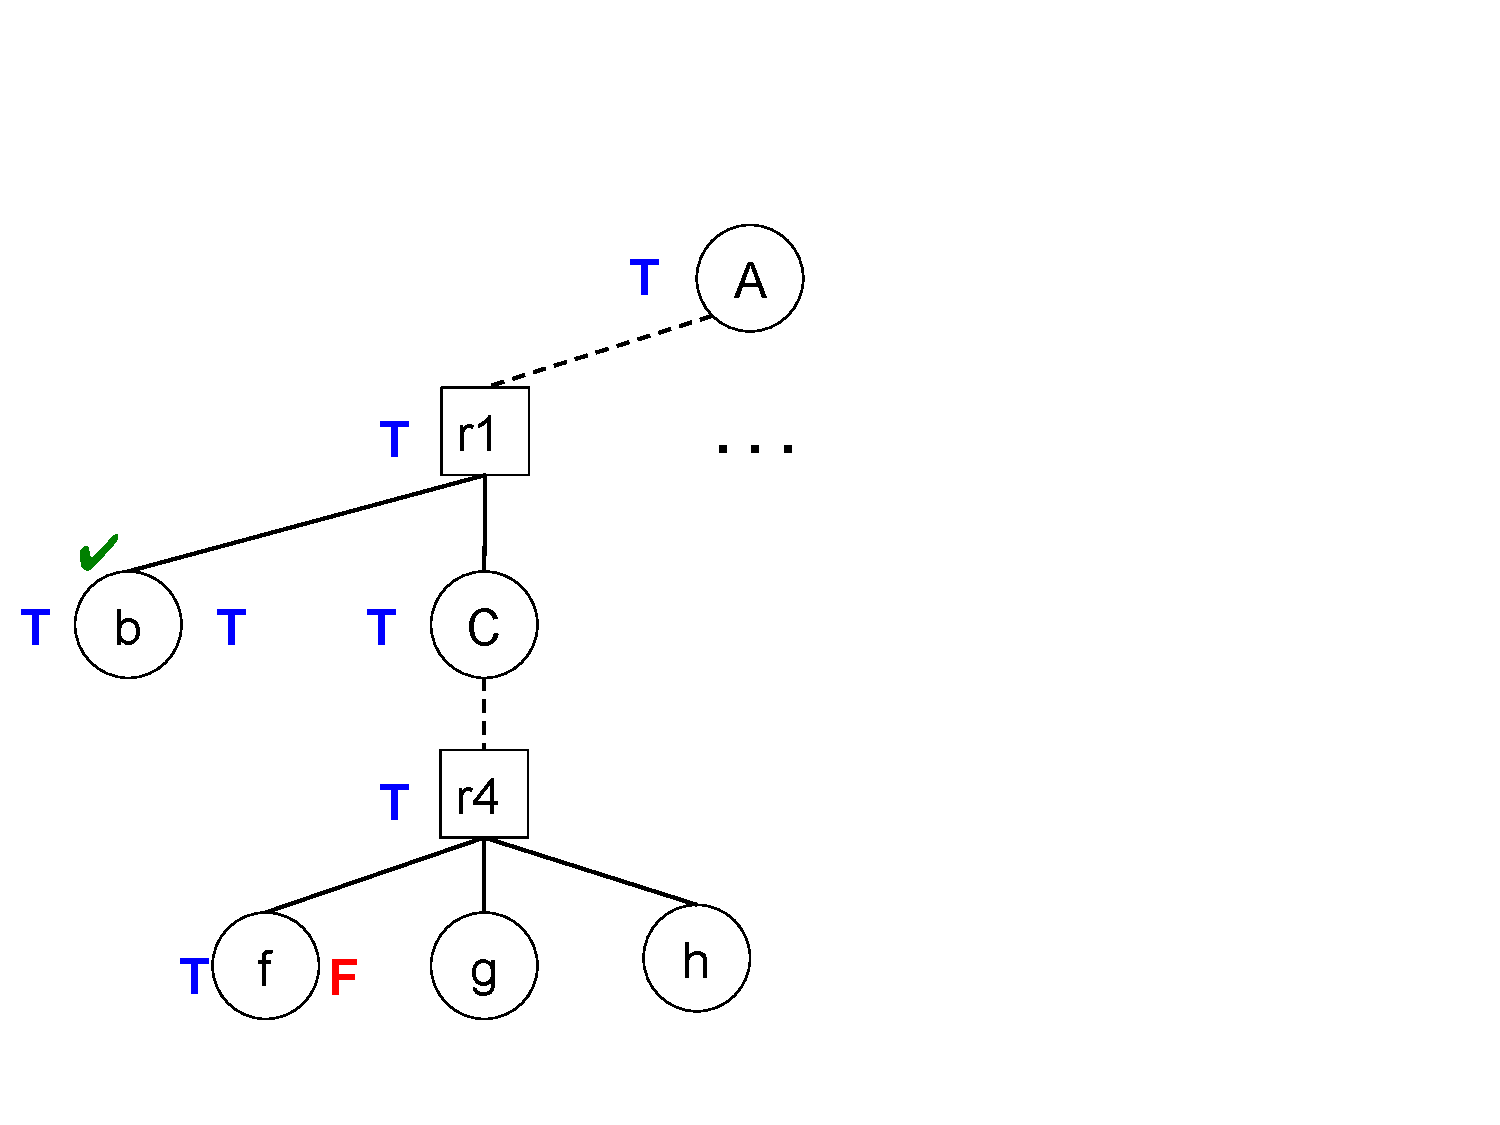
\includegraphics[height=1.3in]{figs/postcondition}}
\vskip 8pt 
\defig{postcondition}{Failed postcondition}
\end{subfigure}
\hfill
\begin{subfigure}{1in}
\centerline{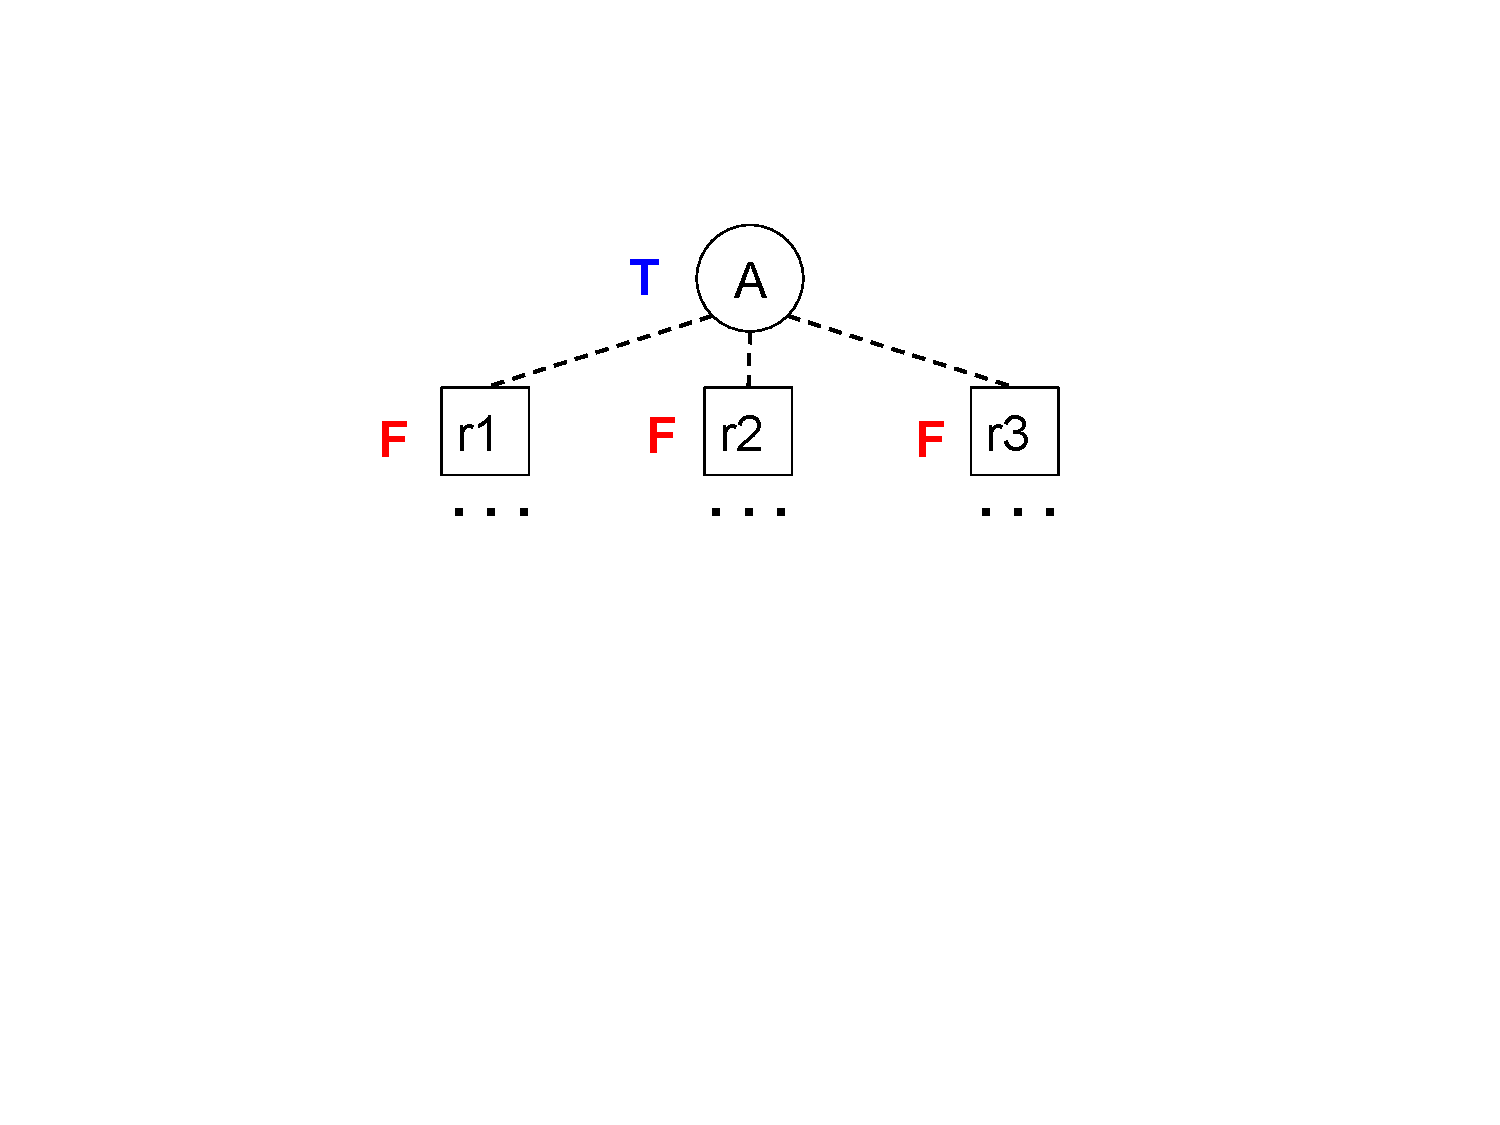
\includegraphics[height=1.3in]{figs/applicability}}
\vskip -2pt
\defig{applicability}{Failed applicability conditions}
\end{subfigure}
\vskip 4pt 
\defig{breakdowns}{Examples of the three types of breakdown in reactive HTN execution.} 
\end{figure}

\fig{breakdowns} summarizes the three types of execution breakdowns
that are possible in reactive HTN execution.  The motivating example
in \sect{motivating} was a failed precondition, as in
\fig{precondition}.  Notice that this taxonomy does not distinguish
between different possible underlying causes of a breakdown.  A
breakdown can be caused by an external, i.e., unmodeled, agency
unexpectedly changing the environment (e.g., the wind in
\sect{motivating}); or it can be due to a programming bug, such as
incorrect tree structure or an incorrectly coded condition.  The fact
these different causes are indistinguishable in the breakdown is
an inherent limitation of reactive HTNs.

\defsubsection{algorithm}{Plan Recovery Algorithm}

\noindent The most significant generalization of the plan recovery
algorithm over the motivating example in \sect{motivating} concerns
the choice of final state for the linear planning problem.  In the
example (see \fig{planning}), the final state is the failed
precondition of the walkthru primitive.  However, there are other
recovery possibilities that might also make sense.  

For example, suppose there was a symbolic postcondition on walkthru
that specified that the robot is located in the room on the other side
of the door.  After the breakdown, another way to recover could be for
the robot to successfully find a plan (using other operators than just
unlock and open) to achieve this condition, e.g., by going out another
door of the current room and taking a different hallway to the
original destination room.  We will call this process making the
postcondition of walkthru the {\em target} of a candidate recovery
planning problem.

Continuing with this line of thought, suppose that there was no
symbolic postcondition provided for walkthru, but the symbolic
postcondition of Navigate specified the desired location of the robot.
In that case, the postcondition of Navigate would be a good candidate
recovery target.

Similarly, suppose the original breakdown in the example had instead
occurred due to the postcondition of unlock failing.  In this
situation, the symbolic precondition of walkthru and the symbolic
postconditions of walkthru and Navigate, if they are provided, are
still good recovery targets.

Based on this reasoning, in the algorithm below we consider the
largest possible set of pre- and postconditions in the tree as
candidate recovery targets, excluding only those that have already
been used in the execution process and have evaluated to true.  We
suspect this is an over-generalization, but need more practical
experience to determine a better approach.

The recovery target issue for applicability conditions is
somewhat different.  The only time that an applicability
condition should be a recovery target is when its and all of its
siblings' conditions have evaluated to false, as in
\fig{applicability}.
	
\begin{figure}[t]
  
  \begin{algorithmic}[1]\small
    
    \Procedure{Execute}{$htn$}
      \While{$htn$ is not completed} 
       \State $current\gets$ next executable node in $htn$
       \If{$current\neq null$} execute $current$
       \Else\hskip 0.1in [breakdown occurred]
         \State $initial\gets$ symbolic description of current world state
         \State $candidates\gets FindCandidates(htn)$
         \State sort $candidates$ by distance from $current$
         \For{$final \in candidates$}
           \State $plan\gets SymbolicPlanner(initial,final)$
           \If{$plan\neq null$}
             \State splice $plan$ into $htn$ between $current$ and $final$
             \State \textbf{continue} while loop above
           \EndIf
         \EndFor
         \State Recovery failed!
        \EndIf
      \EndWhile
    \EndProcedure
\Statex
    \Procedure{FindCandidates}{$task$}
      \State $conditions\gets\emptyset$
      \State $pre\gets$ symbolic precondition of $task$
      \If{$pre\neq null\;\wedge$ procedural prec of $task$ has not evaluated to true}
        \State add $pre$ to $conditions$\EndIf
      \State $post\gets$ symbolic postcondition of $task$
      \If{$post\neq null\;\wedge$ procedural postc of $task$ has not evaluated to true}
        \State add $post$ to $conditions$
      \EndIf
      \State $applicables\gets\emptyset$
      \State $allFalse\gets true$
      \For{$decomp \in$ children of $task$}
        \For{$task\in$ children of $decomp$} $FindCandidates(task)$
        \EndFor 
        \If{$allFalse$}
          \If{procedural appl condition of $decomp$ has evaluated to false}
             \State $app\gets$ symbolic applicability condition of $decomp$
             \If{$app\neq null$} add $app$ to $applicables$\EndIf
          \Else $\;allFalse\gets$ false
          \EndIf 
        \EndIf
      \EndFor
      \If{$allFalse$} add $applicables$ to $conditions$
      \EndIf
      \State\Return $conditions$
    \EndProcedure 
    
  \end{algorithmic}
  \vskip 8pt
  \defig{pseudo}{Pseudocode for hybrid reactive HTN execution and recovery system.}
\end{figure} 

\fig{pseudo} shows the pseudocode for the hybrid system we
have designed.  The toplevel procedure, {\sc Execute}, executes an
HTN until either it is successfully completed, or there is a breakdown
with no possible recovery.  The plan recovery algorithm starts at line
5.  The main subroutine, {\sc FindCandidates}, recursively walks the
HTN tree, accumulating candidate target conditions for the
recovery planning.  Notice that {\sc SymbolicPlanner} is not defined
here, since any symbolic linear planner can be used (our
implementation is described in \sect{evaluation}).  Notice also that
since the set of operators used for symbolic planning doesn't change
during execution of the HTN, it is not an explicit argument to the
symbolic planner (see further discussion regarding symbolic operators
in \sect{methodology}).

In more detail, notice on line 6 that our approach requires a method
for computing from the current world state an initial state
representation in the formalism used by the symbolic planner.  For
example, for the STRIPS planner in \sect{motivating} this means that
for every feature, such as ``open,'' there must be an associated
procedure, such as ``isOpen(),'' to compute its value in the current
world state. This association is a basic part of the hybrid modeling
methodology discussed in next section.

Notice on line 8 that the candidate conditions are sorted by distance
from the current node in the tree (closest first), using a simple
metric such as the length of the shortest path between them in the
undirected graph.  The reason for this is to give preference to
recovery plans that keep more closely to the structure of the original
HTN.  We do not yet have any experience with how well this heuristic
works in practice.

Finally in {\sc Execute}, notice on line 12 that when a recovery plan
is found, it must be properly spliced into the HTN.  In the simple
example in \fig{recover}, this is merely a matter of inserting a
sequence of nodes as children of the common parent between the initial
and final nodes.  However, if the initial and final nodes are more
distant in the tree, more complicated changes are needed to replace
the intervening tree structure with the new plan.

The code in the definition of {\sc FindCandidates} closely follows the 
discussion above regarding possible target conditions. 

\defsubsection{methodology}{Modeling Methodology}

\noindent The hybrid system described above tries to take advantage of
whatever symbolic knowledge is provided by the HTN author.  Notice
that for the pre- or postcondition of each task node there are four
possibilities: no specified condition, only a procedural condition,
only a symbolic condition, or both.  Since applicability conditions
are not optional, there are only two possibilities for decomposition
nodes: only a procedural condition, or a procedural and a symbolic
condition.

As we have argued earlier, symbolic modeling is very difficult in
general.  The reason an author is using a reactive HTN in the first
place is likely because it was not practical to fully model the domain
symbolically.  Two key methodological issues are therefore where to
best invest whatever effort is available for symbolic modeling, and
how to make the overall process of mixed procedural and symbolic
modeling as convenient as possible for the HTN author. We will share
some ideas below, but this is the area in which our work is also
preliminary.

Our initial intuition, illustrated by the example in
\sect{motivating}, is to concentrate symbolic modeling on the
primitive tasks.  This is because we expect symbolic plan recovery to
be most successful as a local planning strategy.

Which pre- and postconditions are provided symbolically also has
implications for the set of operators used by the symbolic planner.
Only a task with both a symbolic precondition and postcondition can be
included in the operator set.  However, the planning operators need
not be restricted to primitive tasks.  If an abstract task is fully
specified symbolically, it can in principle be included in a linear
recovery plan by using its already defined decompositions (and hoping
they are appropriate in the new context).

Finally, we believe there is the opportunity for tools to make the
hybrid modeling process less onerous.  For example, we are planning a
simple design-time tool that recognizes common coding conventions,
such as in \fig{procedures}, and automatically produces corresponding
symbolic conditions, such as in \fig{features}.  Run-time tools can
also keep track of breakdowns and advise where additional symbolic
knowledge may be useful.

\defsection{evaluation}{Implementation and Evaluation}


\begin{floatingfigure}{2.5in}
\centerline{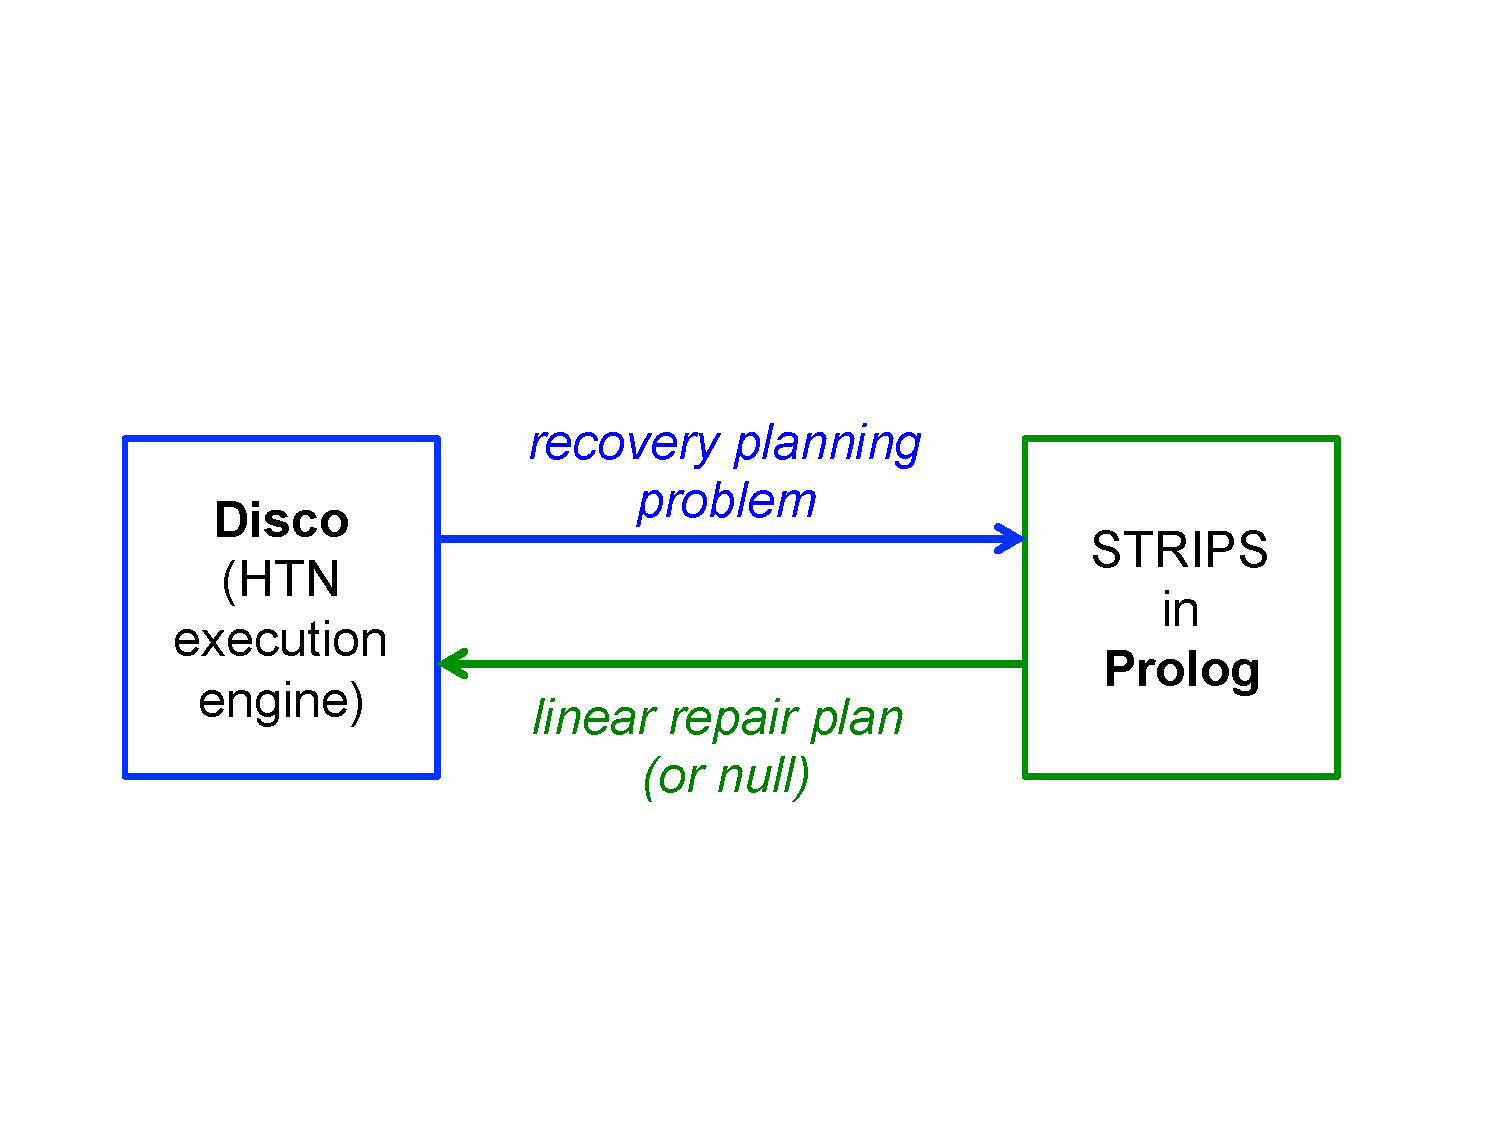
\includegraphics[width=2.4in]{figs/discolog}}
\defig{discolog}{Discolog implementation.}
\end{floatingfigure} 

\noindent We have implemented the hybrid system described above in
pure Java (see \fig{discolog}) using the ANSI/CEA-2018 standard
\cite{CETask} for reactive HTNs and Disco \cite{RichSidner2012} as the
HTN execution engine.  For the symbolic planner, we have used a simple
implementation of STRIPS running in a pure Java implementation of
Prolog.\footnote{See \url{http://tuprolog.apice.unibo.it}} Using
Prolog will facilitate adding additional symbolic reasoning rules to
the planning process.

The ultimate evaluation of our proposed new approach is to
build several agents that operate in complex, dynamic real-world
environments and to see how easy they were to build and how robustly
they performed.  In the meantime, however, we tested our system
on synthetically generated HTNs with different levels of symbolic
knowledge.  Our simple hypothesis was that the more symbolic knowledge
provided, the better the recovery algorithm would perform.

\fig{results} shows the results of our experiments, which confirmed
this hypothesis.  We tested trees of two RxSxD sizes, 3x3x3 and 1x5x4,
where R is the decomposition (recipe) branching factor, S is task
(step) branching factor, and D is the task depth (see \fig{dimen}).
For each test, we randomly sampled from the very large space (millions) of all
possible combinations of symbolic knowledge at three overall levels:
25\%, 50\% and 75\% (percentage of conditions in the tree that are
symbolically specified).  We did not test larger trees because the
experimental running times became too long.

\begin{figure}[t]
\centering
\begin{subfigure}{2.3in}
\centerline{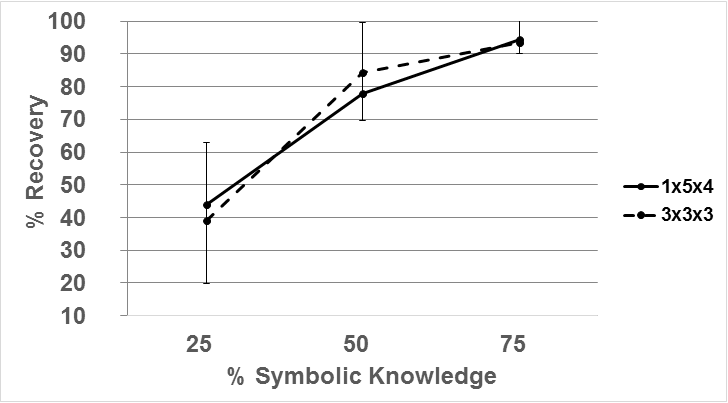
\includegraphics[width=2.3in]{figs/recovery}}
\vskip 8pt 
\defig{recovery}{Recovery/breakdown ratio}
\end{subfigure}
\hfill
\begin{subfigure}{2.3in}
\centerline{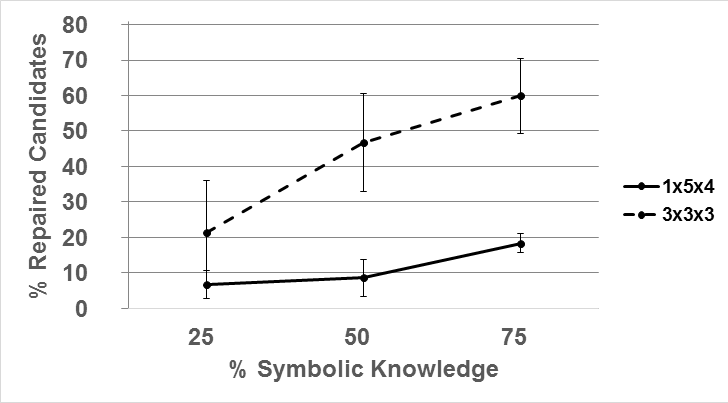
\includegraphics[width=2.3in]{figs/candidates}}
\vskip 8pt 
\defig{candidates}{Proportion of candidates repaired}
\end{subfigure}
\vskip 6pt
\defig{results}{Results of testing on synthetically generated HTNs with different levels of symbolic knowledge.}
 \end{figure}

\begin{floatingfigure}{1.25in}
\centerline{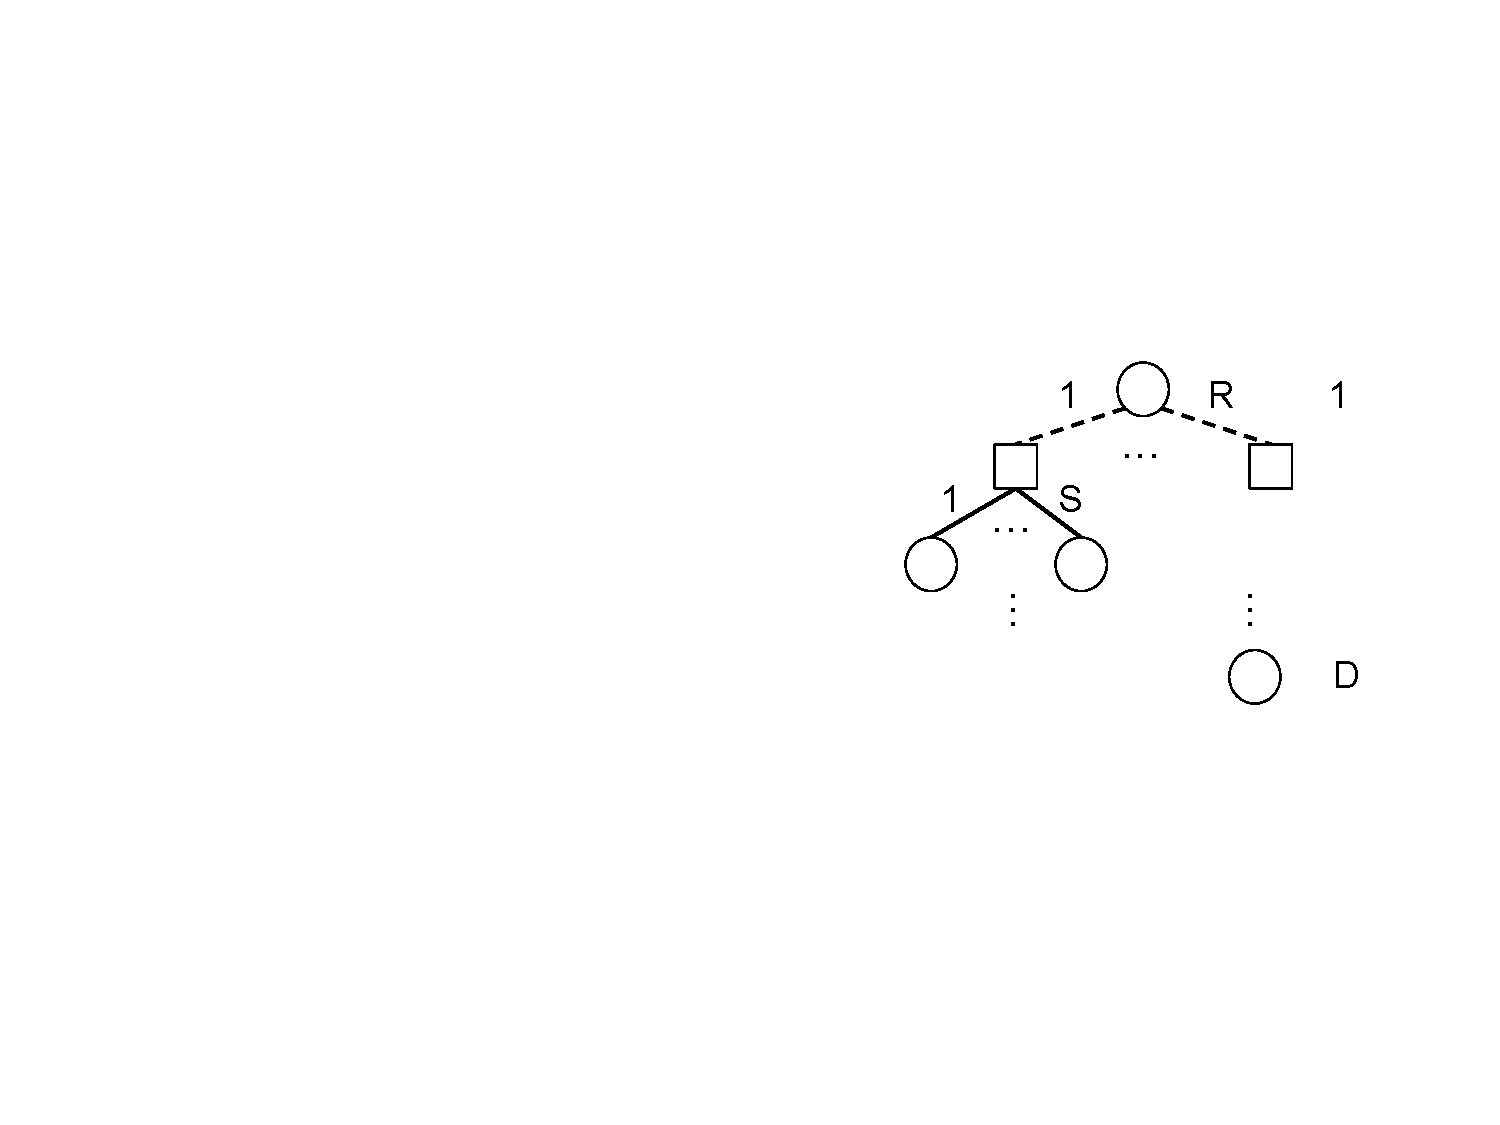
\includegraphics[width=1.2in]{figs/dimen}}
\vskip 4pt
\defig{dimen}{RxSxD}
\end{floatingfigure} 

\fig{recovery} graphs how the proportion of breakdowns that are
successfully recovered increases as the symbolic knowledge
increases. In \fig{candidates}, we were interested in the proportion
of planning problems submitted to the planner which it solved, which
also increased as the symbolic knowledge increased.  (For this
experiment, we made a small modification to the algorithm to prevent it
from stopping at the first solved problem.)

\vskip 4pt
\bibliographystyle{plain}
\bibliography{abbrevs,Library}
\end{document}
